\chapter{The current calculation problem}

In many physical and engineering problems the real interesting variable of the conservation law is the flux in the domain or on specific surfaces and boundaries. The study of micro and nano electronics devices doesn't except this observation, in fact most of all models are oriented to obtain a satisfactory description of the current density.
 We know that the primal and not mixed formulation for  the continuity equation doesn't resolved  the flux density. The conseguence of this fact is a binding post-processing of the quantities computed in order to reconstruct the current density of electrons and holes.
It's evident which this part covers a lead role in the device simulation: 
as we are satisfied of the impressive results of the finite element scheme, it will be reather regrettable to lost the accuracy of our simulation during the computation of the current density.
About this question many academics propose different solutions and  the relative literature is boundless.
 
 
% Nevertheless the problem shows various aspects to take into account, among these there are some which every good method should be respect:	
% \begin{itemize}
% \item reduced computational cost;
% \item easy extension to 3D simulation;
% \item detains some useful properties like orthogonal conservation across a generic surface of the domain;
% \item preserve consistency with the numerical scheme adopted.
% \end{itemize}
% It's not trivial ensure everyone of these points, thus move on toward a unique choice of a method is a delicate matter. 
 
In section \ref{sec: carrier transport} we saw that there exist three way to represent the current density inside a semiconductor device. However each one of these formulas is affected by several numerical issues. We'll investigate this features in order to propose appropriate treatments of the current density computation.

Easily we can exlude the \textit{Slotboom equation} from our consideration. As we already highlighted this formula has relevant properties which make really simple the wellposedness of the continuity equation, however the exponential dependency by the factor $\varphi / V_{th}$ causes unavoidable numerical instability. Therefore we don't consider at priori equation \referenzaeq{eq: Jn slotboom} and \referenzaeq{eq: Jp slotboom} as a way to compute the current density.

We'll center our analysis on the \textit{Drif-Diffusion formula} and the \textit{Quasi Fermi formula}. Finally we'll present two revisions of these expressions in order to fix the numerical weakness.

\section{Standard approaches}

Let us introduce some useful notations: $k$ subscript refers to a quantity defined on elements, while $h$ subscript refers to a quantity defined on verticies. As we used the discrete space $X_h^1$ the solutions $\varphi_h$, $n_h$ and $p_h$ are linear continuous functions. If we refer to \referenzaeq{eq: Jn DD}, \referenzaeq{eq: Jp DD}, \referenzaeq{eq: Jn qf} and \referenzaeq{eq: Jp qf} it's clear that in order to compute $\vect{J}_n$ and $\vect{J}_p$ a numerical derivative on the solutions must be done. Therefore the current densities are constant element piecewise functions ($\vect{J}_{n,k},\vect{J}_{p,k} \in [X_h^0]^3$). 
Thus the current density lives on a different discretized space, if we want combine the quantities, we have to compute appropriate projection of the solutions
 
 \begin{equation}
 n_k := <n_h>
 \end{equation}

For example this operation could be the standard integral average or the armonic average. 

Another important issue is the computation of the derivatives. For this purpose we implemented a numerical derivation based on the Lagrange polynomial interpolator of the first order

\begin{equation}
\nabla n \simeq \nabla (\Pi^1_h n) = \sum_{i=1}^{N_h} n_i \nabla \psi_i = \nabla_k n_h
\end{equation}
 
Notice that the quantity so calculated lives on the appropriate space.
Now we can discretize equations \referenzaeq{eq: Jn DD}, \referenzaeq{eq: Jp DD}, \referenzaeq{eq: Jn qf} and \referenzaeq{eq: Jp qf} as follows

\begin{align}
\vect{J}_n^k &= -q<n>\mu_n\nabla \varphi + qD_n <n>\nabla n \label{eq: Jn DD discrete}\\ 
\vect{J}_p^k &= -q<p>\mu_p\nabla \varphi - qD_p <p> \nabla p \label{eq: Jp DD discrete} \\
\vect{J}_n^k &= -q<n>\mu_n\nabla \varphi_n \label{eq: Jn qf discrete}\\
\vect{J}_p^k &= -q<p>\mu_p\nabla \varphi_p \label{eq: Jp qf discrete}
\end{align}
 
 
Risultati:
\begin{itemize}
\item Problema del compenso fra apporto di drif e diffusion, infatti zona critica quando questi due contributi diventano rilevanti...instability

\item Formula molto stabile tuttavia problemi agli strati limiti delle concentrazioni (problema condizione di contatto differenti comportamenti a seconda della media utilizzata)

\end{itemize}
 
 
\begin{figure}
\centering

\subfloat[][\emph{Jn}]
{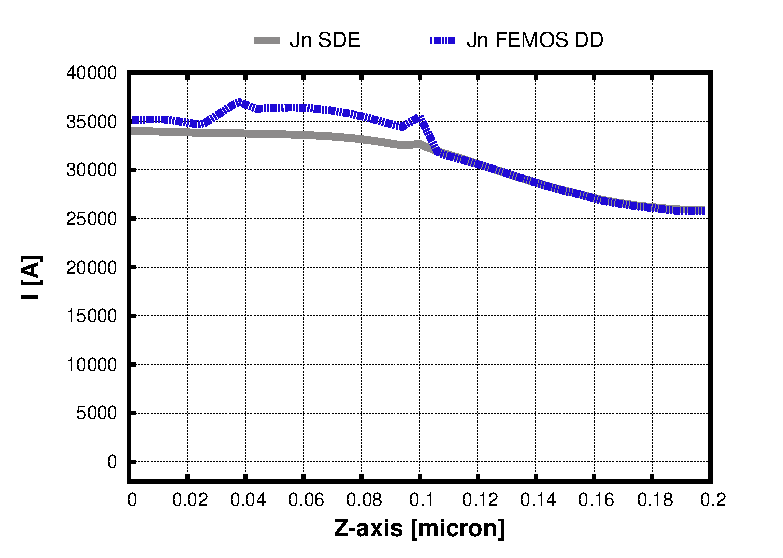
\includegraphics[height=4.5cm]{Corrente/ConfrontiCorrentiBulkJN_SDEVsDD.eps}}
\subfloat[][\emph{Jp}]
{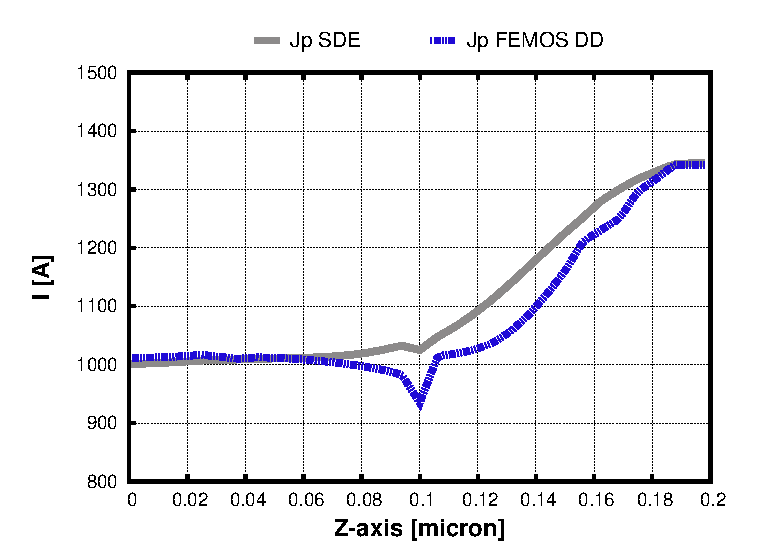
\includegraphics[height=4.5cm]{Corrente/ConfrontiCorrentiBulkJP_SDEVsDD.eps}}

\subfloat[][\emph{Jn}]
{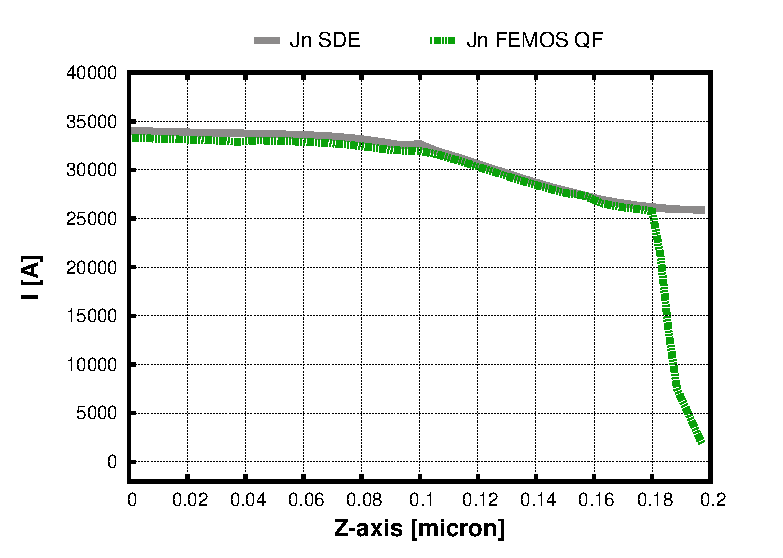
\includegraphics[height=4.5cm]{Corrente/ConfrontiCorrentiBulkJN_SDEVsQF.eps}}
\subfloat[][\emph{Jp}]
{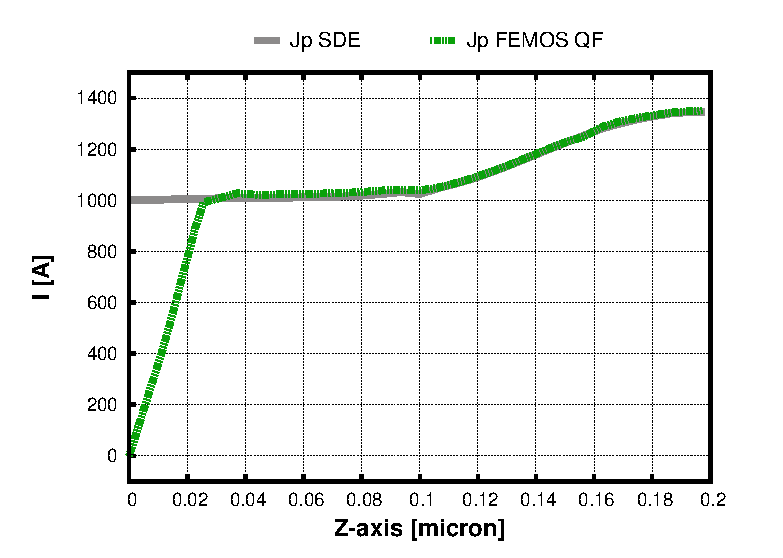
\includegraphics[height=4.5cm]{Corrente/ConfrontiCorrentiBulkJP_SDEVsQF.eps}}


\end{figure} 
 

 
\section{Modified approaches} 
 
 Luckily there's some \textit{main stone} which offers ever a good start point whence achieve new results. Probably the most known and recognized by the inherent literature is the \textit{Sharfetter-Gummel formula}.

\begin{figure}
\centering

\subfloat[][\emph{Jn}]
{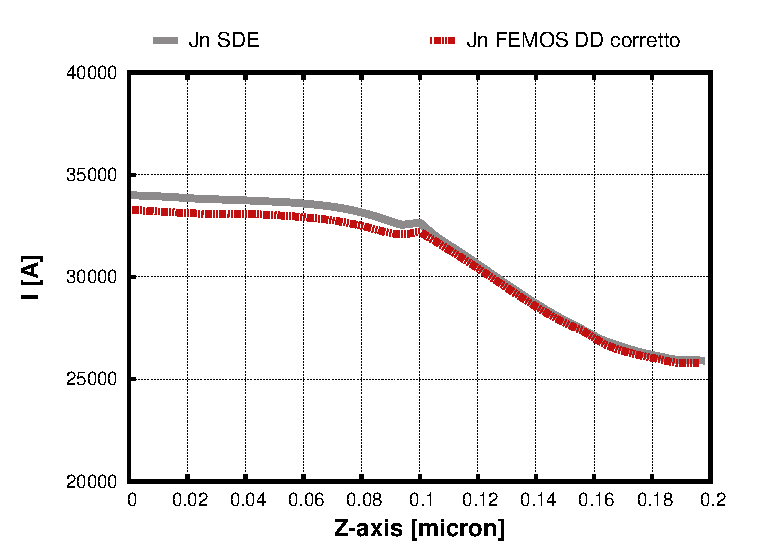
\includegraphics[height=4.5cm]{Corrente/ConfrontiCorrentiBulkJN_SDEVsDDcorretto.eps}}
\subfloat[][\emph{Jp}]
{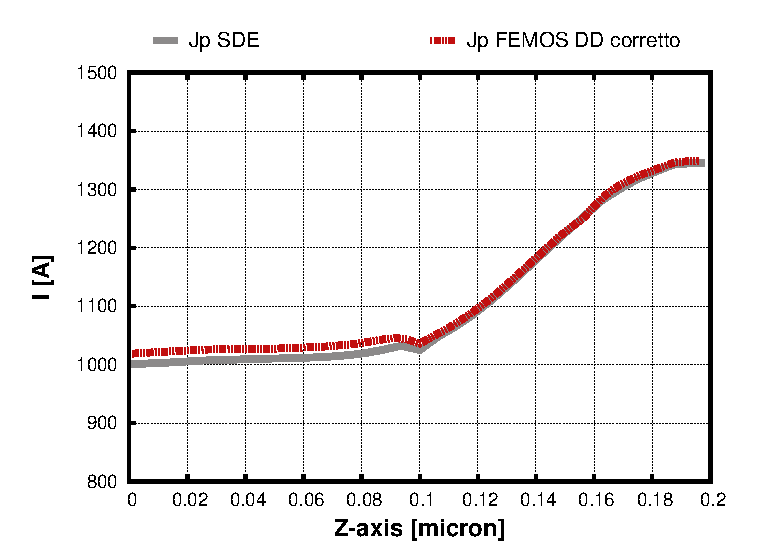
\includegraphics[height=4.5cm]{Corrente/ConfrontiCorrentiBulkJP_SDEVsDDcorretto.eps}}

\subfloat[][\emph{Jn}]
{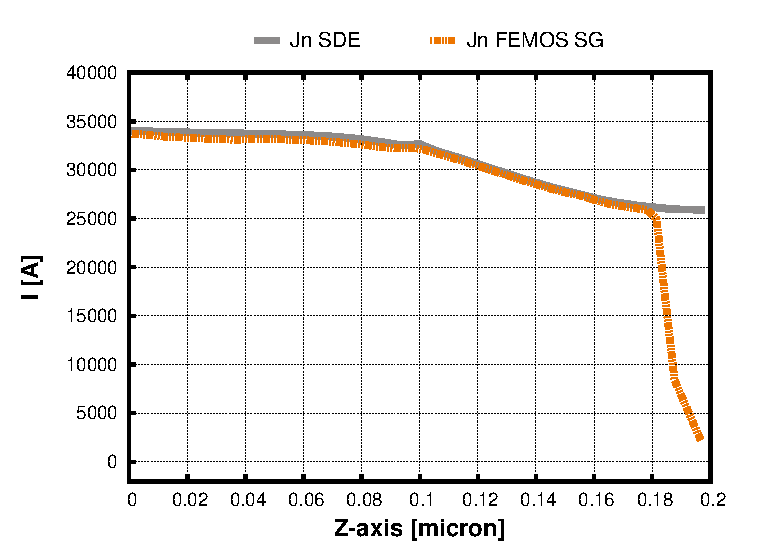
\includegraphics[height=4.5cm]{Corrente/ConfrontiCorrentiBulkJN_SDEVsSG.eps}}
\subfloat[][\emph{Jp}]
{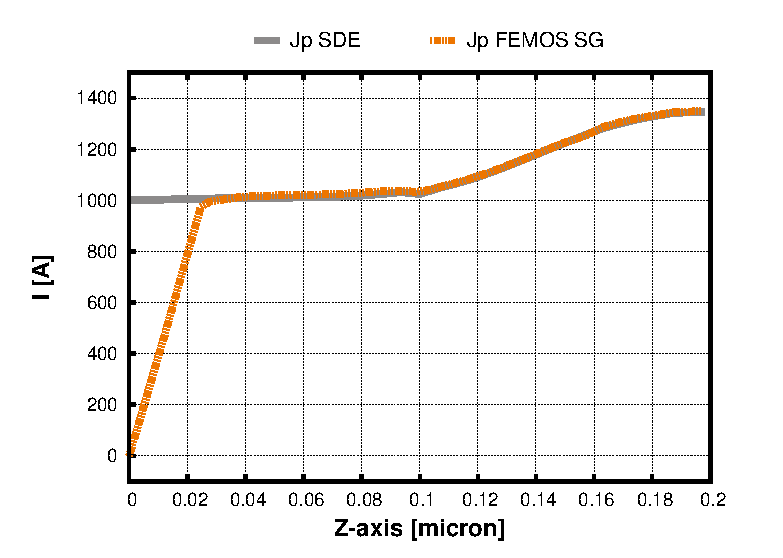
\includegraphics[height=4.5cm]{Corrente/ConfrontiCorrentiBulkJP_SDEVsSG.eps}}


\end{figure} 

\section{Scharfetter-Gummel formula}

Consider the resolution of the continuity equation along a monodimensional domain. For the sake of simiplicity we contemplate a uniform partition (this hypotesis is not necessary for a more generic analysis). Moreover on every nodes is defined the electrostatic potential $\varphi$, and on every elements the relative electrostatic field $\vect{E}$. In order to avoid redundant considerations and calculuses, we proceed with our analysis considering only the current density of electrons ($\vect{J}_n$).

 In 1969 D. Scharfetter and H.K. Gummel (two scientists of Bell Labs), introduced a formula to compute the current density in this case, given $\varphi$ and the density solution ($n$) on every nodes. This innovative approach led for the twenty years to follow every simulation which contemplates electric-devices. 
 
We know that the constituve law is composed by a drift component, which depends on the electric field, and a diffusion component, which depends on the variation of the carrier density. Consider a generic element $K$, we define the drop in voltage $\Delta \varphi^k=\varphi_{i+1}-\varphi_{i}$. There are three possible situations which are well explain in the picture:
\begin{itemize}
\item $\Delta \varphi \gg0$, mainly drift component from right to left 
\item $\Delta \varphi \ll0$, mainly drift component from left to right
\item $\Delta \varphi \simeq 0$, mainly diffusion component
\end{itemize} 
 
 
\begin{center}

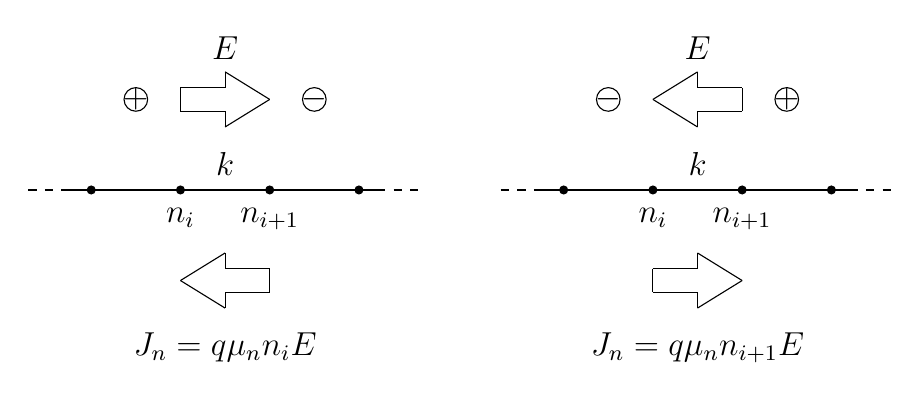
\begin{tikzpicture}
[scale=1.0]
%Solid line
\def\ax{0.5}
\def\ay{0}
\def\bx{4.5}
\def\by{0}

\def\delta{0.3}

%Dash line
\def\cx{0}
\def\cy{0}
\def\dx{5}
\def\dy{0}

\def\Np{3}
\def\step{\bx/\Np-\ax/\Np-2*\delta/\Np}
\def\halfstep{0.5*\bx/\Np-0.5*\ax/\Np-\delta/\Np}

\draw [dashed] (\cx,\cy)--(\dx,\dy);
\draw [thick](\ax,\ay)--(\bx,\by);

\draw [black,draw, fill=black] (\ax+\delta,\ay) circle [radius=0.05];
\draw [black,draw, fill=black] (\ax+\delta+\step,\ay) circle [radius=0.05];
\draw [black,draw, fill=black] (\ax+\delta+\step+\step,\ay) circle [radius=0.05];
\draw [black,draw, fill=black] (\ax+\delta+\step+\step+\step,\ay) circle [radius=0.05];

\draw [thick] (\ax+\delta +\step+\halfstep,\ay+0.05) node[above]{\large $k$};
\draw [thick] (\ax+\delta+\step,\ay-0.1) node[below]{\large $n_{i}$};
\draw [thick] (\ax+\delta+\step + \step,\ay-0.1) node[below]{\large $n_{i+1}$};


\draw [black,draw] (\ax+\delta+\halfstep,\ay+1.15) circle [radius=0.15];
\draw [black,draw] (\ax+\delta+\step + \step + \halfstep,\ay+1.15) circle [radius=0.15];
\node at (\ax+\delta + \halfstep,\ay+1.15){\large $+$};
\node at (\ax+\delta +\step + \step + \halfstep,\ay+1.15){\large $-$};

\node at (\ax+\delta +\step + \halfstep,\ay+1.8){\large $\vect{E}$};
\node at (\ax+\delta +\step + \halfstep,\ay-2.0){\large $\vect{J}_n=q\mu_n n_{i}\vect{E}$};

%Freccia
\draw (\ax+ \delta + \step,\ay+1)--(\ax+\delta+\step+\halfstep,\ay+1);
\draw (\ax+\delta + \step,\ay+1.3)--(\ax+\delta+\step+\halfstep,\ay+1.3);
\draw (\ax+\delta+ \step,\ay+1)--(\ax+\delta+\step,\ay+1.3);
\draw (\ax+\delta + \step +\halfstep,\ay+1.3)--(\ax+\delta+\step+\halfstep,\ay+1.5);
\draw (\ax+\delta + \step +\halfstep,\ay+1)--(\ax+\delta+\step+\halfstep,\ay+0.8);
\draw (\ax+\delta + \step +\halfstep,\ay+1.5)--(\ax+\delta+\step+\step,\ay+1.15);
\draw (\ax+\delta + \step +\halfstep,\ay+0.8)--(\ax+\delta+\step+\step,\ay+1.15);

%Freccia
\draw (\ax+ \delta + \step +\halfstep,\ay-1)--(\ax+\delta+\step +\step,\ay-1);
\draw (\ax+\delta + \step + \halfstep,\ay-1.3)--(\ax+\delta+\step + \step,\ay-1.3);
\draw (\ax+\delta+ \step + \step,\ay-1)--(\ax+\delta+\step+\step,\ay-1.3);

\draw (\ax+\delta + \step +\halfstep,\ay-1.3)--(\ax+\delta+\step+\halfstep,\ay-1.5);
\draw (\ax+\delta + \step +\halfstep,\ay-1)--(\ax+\delta+\step+\halfstep,\ay-0.8);
\draw (\ax+\delta + \step +\halfstep,\ay-1.5)--(\ax+\delta+\step,\ay-1.15);
\draw (\ax+\delta + \step +\halfstep,\ay-0.8)--(\ax+\delta+\step,\ay-1.15);


%Solid line
\def\ax{6.5}
\def\ay{0}
\def\bx{10.5}
\def\by{0}

\def\delta{0.3}

%Dash line
\def\cx{6}
\def\cy{0}
\def\dx{11}
\def\dy{0}

\def\Np{3}
\def\step{\bx/\Np-\ax/\Np-2*\delta/\Np}
\def\halfstep{0.5*\bx/\Np-0.5*\ax/\Np-\delta/\Np}

\draw [dashed] (\cx,\cy)--(\dx,\dy);
\draw [thick](\ax,\ay)--(\bx,\by);

\draw [black,draw, fill=black] (\ax+\delta,\ay) circle [radius=0.05];
\draw [black,draw, fill=black] (\ax+\delta+\step,\ay) circle [radius=0.05];
\draw [black,draw, fill=black] (\ax+\delta+\step+\step,\ay) circle [radius=0.05];
\draw [black,draw, fill=black] (\ax+\delta+\step+\step+\step,\ay) circle [radius=0.05];

\draw [thick] (\ax+\delta +\step+\halfstep,\ay+0.05) node[above]{\large $k$};
\draw [thick] (\ax+\delta+\step,\ay-0.1) node[below]{\large $n_{i}$};
\draw [thick] (\ax+\delta+\step + \step,\ay-0.1) node[below]{\large $n_{i+1}$};

\draw [black,draw] (\ax+\delta+\halfstep,\ay+1.15) circle [radius=0.15];
\draw [black,draw] (\ax+\delta+\step + \step + \halfstep,\ay+1.15) circle [radius=0.15];
\node at (\ax+\delta + \halfstep,\ay+1.15){\large $-$};
\node at (\ax+\delta +\step + \step + \halfstep,\ay+1.15){\large $+$};

\node at (\ax+\delta +\step + \halfstep,\ay+1.8){\large $\vect{E}$};
\node at (\ax+\delta +\step + \halfstep,\ay-2.0){\large $\vect{J}_n=q\mu_n n_{i+1}\vect{E}$};

%Freccia
\draw (\ax+ \delta + \step +\halfstep,\ay+1)--(\ax+\delta+\step +\step,\ay+1);
\draw (\ax+\delta + \step + \halfstep,\ay+1.3)--(\ax+\delta+\step + \step,\ay+1.3);
\draw (\ax+\delta+ \step + \step,\ay+1)--(\ax+\delta+\step+\step,\ay+1.3);
\draw (\ax+\delta + \step +\halfstep,\ay+1.3)--(\ax+\delta+\step+\halfstep,\ay+1.5);
\draw (\ax+\delta + \step +\halfstep,\ay+1)--(\ax+\delta+\step+\halfstep,\ay+0.8);
\draw (\ax+\delta + \step +\halfstep,\ay+1.5)--(\ax+\delta+\step,\ay+1.15);
\draw (\ax+\delta + \step +\halfstep,\ay+0.8)--(\ax+\delta+\step,\ay+1.15);

%Freccia
\draw (\ax+ \delta + \step,\ay-1)--(\ax+\delta+\step+\halfstep,\ay-1);
\draw (\ax+\delta + \step,\ay-1.3)--(\ax+\delta+\step+\halfstep,\ay-1.3);
\draw (\ax+\delta+ \step,\ay-1)--(\ax+\delta+\step,\ay-1.3);
\draw (\ax+\delta + \step +\halfstep,\ay-1.3)--(\ax+\delta+\step+\halfstep,\ay-1.5);
\draw (\ax+\delta + \step +\halfstep,\ay-1)--(\ax+\delta+\step+\halfstep,\ay-0.8);
\draw (\ax+\delta + \step +\halfstep,\ay-1.5)--(\ax+\delta+\step+\step,\ay-1.15);
\draw (\ax+\delta + \step +\halfstep,\ay-0.8)--(\ax+\delta+\step+\step,\ay-1.15);

\end{tikzpicture}


\end{center}


With the $Sharfetter-Gummel$ formula it's possibile taking into account every of these situations and solve boundary layer problems which occurs often in presence of strong drift component contribute.

 \begin{equation}
\label{eq: scharfetter gummel 1D electron}
J_n^k=q\frac{D_n}{h}
\left[ n_{i+1}\mathcal{B}\left(\frac{\Delta \varphi^k}{V_{th}}\right)- n_i\mathcal{B}\left(-\frac{\Delta \varphi^k}{V_{th}}\right)\right]  
\end{equation}

In the latter case $\Delta \varphi=0$) the formula became:

\begin{equation}
J_n^k=qD_n\frac{n_{i+1}-n_{i}}{h}
\end{equation}

which is the correct approximation of the current density using $\mathbb{P}_1$ basis. 

Morover many mathematics discover important properties about this method \textcolor{red}{questa parte la vorrei fare meglio}. 
These changes in the direction of the electric field lead to boundary layer problems. It's not possibile afford these situations with a simply upwinding sheme ...

\section{Extension for the 3D case}
 
The extension of this formula for the 3D case is not trivial. We show the method for the computation of the current density of electrons (the extension for the current density of holes is quite similar).
We remark the quasi fermi formula for current density:
\begin{equation}
\label{eq: current density fermi}
\vect{J}_n=-q \mu_n n \nabla \varphi_n
\end{equation}
where $\varphi_n$ is the quasi fermi potential level. Let us write \referenzaeq{eq: current density fermi} in function of potential and in a canonic form:
\begin{equation}
\label{eq: current density canonic form}
\vect{J}_n\dfrac{ exp\left(\dfrac{\varphi_n-\varphi}{V_{th}}\right)}{q \mu_n n_i} + \nabla \varphi_n = 0
\end{equation}

We consider $\vect{J}_n\in[L^2(\Omega)]^3$ and $\varphi_n,\varphi \in H^1(\Omega)$. We are able to multiply \referenzaeq{eq: current density canonic form} with a generic function $\vect{q}\in[L^2(\Omega)]^3$ and then intagrate over the domain $\Omega$:

\begin{equation}
\label{eq: variation form of current density continuos}
\int_\Omega \dfrac{ exp \left( \dfrac{\varphi_n-\varphi}{V_{th}} \right) }{q \mu_n n_i} \vect{J}_n \cdot \vect{q} \, d\Omega
 + \int_\Omega \nabla \varphi_n \cdot \vect{q} \, d\Omega = 0 
\end{equation}


We proceed taking the usual discrete space of the constant elemenwise functions:

\begin{equation}
\label{eq: spaces elementwise constant}
V_h=\left\{ w \in L^2(\Omega) : w|_{K}\in \mathbb{P}_0 \forall K \in \tau_h\right\}
\end{equation}

Now the discrete quantitaties are $\vect{J}_n^h\in[V_h]^3$ and $\nabla \varphi_n^h \in V_h$. We desire produce a system of equation on every elements for the three componente of $\vect{J}_n$, this is possible with a smart choice of the test function $\vect{q}_h \in [V_h]^3$:

\begin{equation}
\label{eq: form of qh}
\vect{q}^h_{1,2,3} = \left\{ \begin{bmatrix} 1 \\ 0 \\ 0 \end{bmatrix}  \begin{bmatrix} 0 \\ 1 \\ 0 \end{bmatrix}  \begin{bmatrix} 0 \\ 0 \\ 1 \end{bmatrix}  \right\}
\end{equation}

From \referenzaeq{eq: variation form of current density continuos} we obtain the sequent system of equations defined for every element of the mesh:

\begin{equation}
\label{eq: variation form of current density}
\int_K \dfrac{ exp \left( \dfrac{\varphi_n-\varphi}{V_{th}} \right) }{q \mu_n n_i} \vect{J}_n^h \cdot \vect{q}^h_i \, dK
 + \int_K \nabla \varphi_n^h \cdot \vect{q}^h_i \, dK = 0 \psp{10} \forall i=1,2,3
\end{equation}

Operating the intagration we obtain the sequent formula for the current density components:

\begin{equation}
\label{eq: first formula for J}
[\vect{J_n}]_i = - \mathbb{H}_K \left( q \mu_n n_i exp \left( \dfrac{\varphi-\varphi_n}{V_{th}} \right)  \right) \dfrac{\partial \varphi_n^h}{\partial x_i} \psp{5} i = 1...d \psp{5} \forall K \in \tau_h
\end{equation}

where $\mathbb{H}_K(f)$ is the armonic average on the elment $K$ of the function $f$.

Although resolve the armonic average with a comlete 3D integration may be expensive in calculation time and propably not necessary. One approximation of this integral would be pass from a 3D integration to 1D integration along one edge of the element $K$.
\begin{equation}
\label{eq: approzimation from 3D to edge}
\left(\dfrac{\int_K f^{-1} \, dK}{|K|} \right)^{-1} \simeq \left(\dfrac{\int_{e*} f^{-1} \, de}{|e^*|} \right)^{-1}
\end{equation}
  The approximation \referenzaeq{eq: approzimation from 3D to edge} is valid if we consider the correct edge.


Consider a quantity defined on the verteces:
\begin{equation}
\label{eq: differenza tra pot e qf}
\Phi := \varphi - 	\varphi_n
\end{equation}
which is the difference between the electrostatic potential and the quasi fermi potential level. Now for every element consider two vertices: $\vect{x}_m$ s.t. $\Phi(\vect{x}_m)=\Phi_m := min_K(\Phi)$ and $\vect{x}_M$ s.t. $\Phi(\vect{x}_M)=\Phi_M:=max_K(\Phi)$. Obviously it exists only one edge which connects these two points and on this one we perform the 1D integration \referenzaeq{eq: approzimation from 3D to edge}. First of all as we reduce the dimension is feasible to represent $\sigma(\vect{x})$ in a easier mode as follows:

\begin{equation}
\sigma_n(s) = q \mu_n n_i exp\left( \Phi_m + (\Phi_M-\Phi_m)\dfrac{s-s_m}{|e^*|} \right)
\end{equation}

where $s \in [s_m,s_M]$ is the parameter refered to the edge $e^*$ s.t. $\sigma_n(s_m)=\sigma_n(\vect{x}_m)$ and $\sigma_n(s_M)=\sigma_n(\vect{x}_M)$. We can easily resolve \referenzaeq{eq: approzimation from 3D to edge} with the substitution of variable:
\begin{equation*}
\eta := \dfrac{s-s_m}{|e^*|}
\end{equation*}

this lead us to the sequent steps of integration:

\begin{multline*}
\int_{e^*} \sigma_n^{-1} \, de = |e^*| \int_0^1 \dfrac{exp \left(-\Phi_m - (\Phi_M-\Phi_m)\eta \right)}{q\mu_n n_i} 
 \, d\eta \\
 = |e^*|\dfrac{exp (-\Phi_m)}{q\mu_n n_i} \dfrac{exp ( \Phi_m-\Phi_M)-1}{\Phi_m-\Phi_M} \\
 =  |e^*|\dfrac{exp (-\Phi_m)}{q\mu_n n_i} \dfrac{1}{\mathbf{B}(\Phi_m-\Phi_M)}
\end{multline*}

finally we obtain:
\begin{equation}
\label{eq: finally approzimation 3D to 1D}
\int_{K} \sigma_n^{-1} \, dK \simeq  q \mu_n n_i exp(\Phi_m) \mathbf{B}(\Phi_m-\Phi_M)
\end{equation}

Similar results may be obtained repeating the integration and considering $s_M$ as start point:

\begin{equation}
\int_{K} \sigma_n^{-1} \, dK \simeq  q \mu_n n_i exp(\Phi_M) \mathbf{B}(\Phi_M-\Phi_m)
\end{equation}

Numerical results (\textcolor{red}{qua sarebbe carino fare un po' di test con una parte o l'altra della formula per mettere in crisi}) shows that the best choice is e linea combination of these approzimations as follows:

\begin{equation}
\label{eq: first formula for J}
\vect{J_n}^K = -  q \mu_n  \left[ \dfrac{ n_{min} \mathbf{B}(-\Delta \Phi_{max})  + n_{max}\mathbf{B}(\Delta \Phi_{max})}{2} \right]\nabla \varphi_n^h
\end{equation}
This approach is the natrual extension of the $Sharfetter-Gummel$ formula for the 1D case, indeed it's possible demonstrate the equivalence assuming a monodimensionale domain.


\begin{figure}[!h]
\centering
\subfloat[][\emph{FEMOS}]
{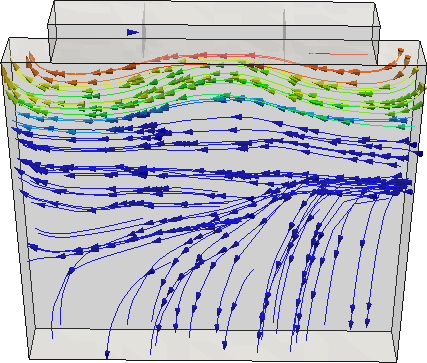
\includegraphics[scale=0.38]{Results/MOS/FEMOS181718_Jn2voltONLYDEVICE.png}}
\hspace{0.5cm}
\subfloat[][]
{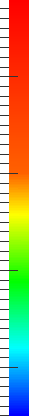
\includegraphics[scale=0.3]{Results/MOS/LegendaArcobalenoVert.png}}
\hspace{0.5cm}
\subfloat[][\emph{SDEVICE}]
{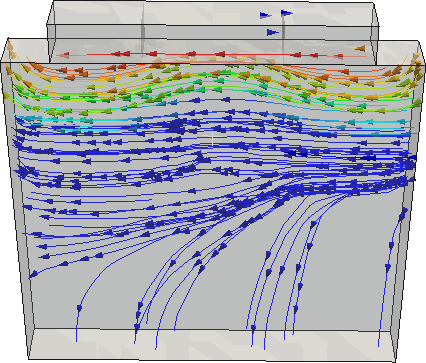
\includegraphics[scale=0.38]{Results/MOS/SDEVICE181718_Jn2voltONLYDEVICE.png}}
\caption{Electron current density Vgate = 2.0 [V].}
\end{figure}

